\PassOptionsToPackage{sols}{handout}
\documentclass[main]{subfiles}
\setcounterrefbeforedot{chapter}{m-ws1-2}
\setcounterrefafterdot{section}{m-ws1-2}
\addtocounter{section}{-1}
\usepackage{solutions}

\begin{document}

\section{Related Rates of Change} \label{ws1-2}

% \begin{objectives}
% You should be able to:

% \begin{itemize}[topsep=0pt,partopsep=0pt,parsep=8pt,itemsep=0pt]

% \item You should be able to apply the Chain Rule like a pro!

% \item You should be able to apply the Chain Rule in more general contexts,
%   such as in a word problem or when given a composition of functions
%   described by graphs or numerical data.

% \item You should understand how logarithms and the Chain Rule can be used
%   to show that the Power Rule $\tfrac{d}{dx} \left( x^n \right) =
%   nx^{n-1}$ holds for any real number $n$.  (In Math Ma, we only proved
%   the Power Rule in the case where $n$ is an integer or $1/2$.)

% \end{itemize} 

% \end{objectives}

\textbf{Key Idea}: Leibniz notation can be used to represent a rate of change with respect to a specific variable.

\begin{enumerate}
\item Many stars, including our sun, will expand to many times their original size as they exhaust their hydrogen fuel. As an analogy, let's consider a rapidly expanding spherical balloon.

As the balloon expands, we determine that the radius $r$ (in centimeters) is related to the elapsed time $t$ (in seconds) by the equation $r=1+2t^2$.

The formula for the volume of a sphere with radius $r$ is $V=\tfrac{4}{3}\pi r^3$.

\begin{enumerate}
\item
\begin{problem}
Write an equation that relates the volume of the sphere $V$ to the elapsed time $t$.
\end{problem}
\pspace{\stretch{0.25}}

\begin{solution}
    If $r$ is related to $t$ through the equation $r=1+2t^2$, and volume is related to radius through the equation $V=\frac{4}{3}\pi r^3$, we can relate volume to time by substituting $1+2t^2$ for $r$ everywhere that $r$ appears in the equation for volume.
    $$V=\frac{4}{3} \pi (1+2t^2)^3$$
\end{solution}
\item
\begin{problem}
What does the symbol $\diff{V}{t}[t=1]$ represent? What is its value, and what are the units?
\end{problem}
\pspace{\vfill}

\begin{solution}
    The symbol $\diff{V}{t}[t=1]$ represents the instantaneous rate of change of volume with respect to time at the specific time $t=1$.\\
    We can find its value by differentiating $V$ with respect to $t$, setting $t$ equal to 1, and then evaluating.\\
    \begin{align*}
        V &=\frac{4}{3} \pi (1+2t^2)^3\\
        \diff{V}{t} &= \frac{4}{3}\pi \cdot 3(1+2t^2)^2\cdot (4t)\\
    \diff{V}{t}[t=1] &= \frac{4}{3}\pi \cdot 3(1+2 (1)^2)^2 \cdot(4(1))\\
    &=\frac{4}{3}\pi\cdot 3(3)^2(4)\\
    &=\frac{4}{3}\pi \cdot (27)(4)\\
    &=4\cdot 4 \cdot 9 \pi\\
    &=144\pi
    \end{align*}
    \fbox{  $\displaystyle \diff{V}{t}[t=1] = 144\pi \text{ cubic centimeters per second}$}
\end{solution}

\item
\begin{problem}
Your classmate wants to find the value of $\diff{V}{t}[r=3]$. Their reasoning is given below.

\textbf{Classmate's reasoning}: 
\begin{enumerate}
    \item The derivative of $V$ is $4\pi r^2$.
    \item We want the derivative when $r=3$, so we should plug in $r=3$.
    \item The value we get is $36\pi$. 
\end{enumerate}

Is their reasoning correct? If not, what is the issue?
\end{problem}
\pspace{\vfill}

\begin{solution}
    Their reasoning is not correct. $\diff{V}{t}[r=3]$ represents the instantaneous rate of change of volume \emph{with respect to time} when the radius is 3. The classmate is differentiating volume with respect to radius, rather than time. We can see this because the original equation describes volume only in terms of $r$.
\end{solution}

\item 
\begin{problem}
Now suppose we don't know the exact relationship between $r$ and $t$. But we know that, when the radius of the balloon is 3\,cm, the radius is increasing at a rate of 4\,cm/s. Is this enough information to determine how fast the volume is changing when the radius is 3\,cm?
\end{problem}
\pspace{\vfill}

\begin{solution}
    Yes, this is enough information, but might not be immediately obvious.
    
    Let's summarize what's been communicated to us: (1) the value of the radius at a specific moment and (2) the rate at which the radius is increasing at that moment as time passes. 
    
    With no further work, this does not determine how volume is changing with respect to time. However, with additional calculations, we can find the rate we're looking for. 
    
    In our discussion of part (c), we found that our classmate was [inappropriately] computing the rate at which volume was changing with respect to the radius. This is now useful!  If we know how much volume is increasing with each cm increase in radius \emph{and} we know the rate at which the radius is increasing per second, the product of these quantities will tell us the rate at which volume is changing with respect to time (which is what we're looking for in this problem).
    
    How is volume is changing with respect to the radius? Since $V = \frac{4}{3} \pi r^3$, then $\diff{V}{r} = 4\pi r^2$. We are told $r=3$ at a specific moment, which means that $\diff{V}{r}[r=3] = 4\pi \cdot 3^2 = 36\pi$ at that moment. In this context, this means that volume is increasing by $36\pi$ cubic centimeters for every centimeter increase in radius at this moment.
    \begin{align*}
        \diff{V}{t}&= \diff{V}{r}\cdot\diff{r}{t}\\
        \diff{V}{t}[r=3]&= \diff{V}{r}[r=3]\cdot\diff{r}{t}[r=3]\\
         \diff{V}{t}[r=3]&= 36\pi\cdot4\\
          \diff{V}{t}[r=3]&= 144\pi \
    \end{align*}
    Even without a specific formula giving us the explicit relationship between $V$ and $t$, we can determine $\diff{V}{t}$ at a particular moment in time if we know (1) the rate at which volume is changing with respect to radius and (2) the rate at which radius is changing with respect to time at that given moment. 
\end{solution}
\end{enumerate}
\end{enumerate}

\pspace{\newpage}

\textbf{Key Idea}: Related variables have related rates of change.

\begin{enumerate}[resume]
\item A charged particle is moving in a uniform magnetic field. As it moves, it follows a curved path described by the equation $x^2+y^2=25$.
\begin{enumerate}
\item
\begin{problem}
Sketch the path of the particle.
\end{problem}
\pspace{\vfill}

\begin{solution}
    The equation $x^2+y^2=25$ describes a circle centered at the origin with radius 5. 

    \begin{center}
        \begin{tikzpicture}
            \begin{axis}[xlabel=$x$,ylabel=$y$, axis equal image, xmin=-5.5, xmax=5.5, ymin=-5.5, ymax=5.5, xtick distance=1, ytick distance=1, xticklabels=\empty, yticklabels=\empty]
                \addplot[domain=0:360] ({5*cos(x)},{5*sin(x)});
            \end{axis}
        \end{tikzpicture}
    \end{center}
\end{solution}
\item 
\begin{problem}
As the particle moves, its $x$-coordinate and $y$-coordinate both change with time. We'll call the respective rates of change $\diff{x}{t}$ and $\diff{y}{t}$. Without using calculus, what can you say about how these rates are related? For example, if $\diff{x}{t}$ is positive, can you say anything about the sign of $\diff{y}{t}$?
\end{problem}
\pspace{\vfill}

\begin{solution}
    We can use our sketch to reason about how the $x$-coordinate and $y$-coordinates change together, which will depend on which part of the circular path we're on. If  $\diff{x}{t}$ is positive, we know this means that the $x$-coordinate is increasing. In the plane, we are moving to the right. Let's look at different parts of the circle: 
    
    If we are in either quadrants I or III, moving to the right along the circular path corresponds with the moving downward, meaning the $y$-coordinate is decreasing or $\diff{y}{t}$ is negative. 
    
    If we are in either quadrants II or IV, moving to the right means we are also moving upward, meaning the $y$-coordinate is increasing, or $\diff{y}{t}$ is positive.  
\end{solution}

\item 
\begin{problem}
The relationship between $x$ and $y$ is $x^2+y^2=25$. Differentiate both sides with respect to $t$ to get a relationship between $\diff{x}{t}$ and $\diff{y}{t}$. Remember, $x$ and $y$ are functions of $t$.
\end{problem}
\pspace{\vfill}

\begin{solution}
We'll begin with our relationship between $x$ and $y$.
    \begin{align*}
x^2+y^2&=25\\
\intertext{Differentiating with respect to $t$, we have:}
2x\cdot \diff{x}{t} + 2y\cdot \diff{y}{t} &= 0
\end{align*}
Now notice that $x$ and $y$ do not have an explicit relationship to $t$. However, we know that $x$ and $y$ are both changing as time passes. Similar to the previous problem, we can determine the rate at which $x^2$ is changing with respect to time by computing the product of the rate at which $x^2$ is changing with respect to $x$ (which is $2x$) and the rate at which $x$ is changing with respect to time (which is $\diff{x}{t}$).  We apply similar reasoning to determine how fast $y^2$ is changing with respect to time: we multiply the rate at which $y^2$ is changing with respect to $y$ (which is $2y$) by the rate at which $y$ is changing with respect to time (which is $\diff{y}{t}$). This is an application of the Chain Rule, which we learned about last semester.
\end{solution}
\item
\begin{problem}
When the particle is at the point $(-4, 3)$, we measure that its $y$-coordinate is decreasing at a rate of 2 units per second. How fast is the particle's $x$-coordinate changing? Does the answer you calculated make sense given the motion of the particle?
\end{problem}
\pspace{\vfill}

\begin{solution}
It's easiest to collect our information. We're told that the particle is at $(-4,3)$, so at this moment in time $x=-4$, $y=3$. We also know  the $y$-coordinate is decreasing at a rate of 2 units per second, so at this moment $\diff{y}{t} = -2$. We are asked for how fast the $x$-coordinate is changing, which is $\diff{x}{t}$. Notice that we have values for all but one quantity in the relationship we found in (c). Let's substitute in our known quantities and solve for $\diff{x}{t}$
    \begin{align*}
    2x\cdot \diff{x}{t} + 2y\cdot \diff{y}{t} &= 0\\
    2(-4)\cdot \diff{x}{t}+2(3)\cdot (-2) &=0\\
    -8\diff{x}{t}-12&=0\\
    -8\diff{x}{t}&=12\\
    \diff{x}{t}&=-\frac{12}{8}\\
    \diff{x}{t}&=-\frac{3}{2}
    \end{align*}
    This means that the $x$-coordinate is decreasing at a rate of $\frac{3}{2}$ units per second. This makes sense because $(-4, 3)$ is in Quadrant II. If the $y$-coordinate is decreasing, it means we are moving downward. Doing that along this circular path means we are moving to the left as well, which means the $x$ coordinate is also decreasing, so we'd expect $\diff{x}{t}$ to be negative. 
\end{solution}
\end{enumerate}

\end{enumerate}
\newpage

\textbf{Key Idea}: Similar figures are related by scaling. Angle measures are the same, side lengths are proportional.

\begin{enumerate}[resume]
\item 
\begin{problem}
In Lesson 1.1, we found that the point $(\sqrt{2}, \sqrt{2})$ is on the graph of $x^2+y^2=4$, shown in figure (a). Using similarity, determine the coordinates of the corresponding points marked in figures (b) and (c).
\end{problem}
\end{enumerate}
\probonly{
\vspace{-18pt}
\begin{center}
    
\includegraphics[width=\textwidth]{tikz/1-2/1-2-isosceles.pdf}
\end{center}
}

\begin{solution}
\begin{center}
\resizebox{\textwidth}{!}{
    \begin{tikzpicture}
  \begin{groupplot}[
    axis equal image,
    xmin=-3.5, xmax=3.5,
    ymin=-3.5, ymax=3.5,
    xtick distance=1, ytick distance=1,
    xlabel={$x$}, ylabel={$y$},
    clip=false,
    group style={group name=my plots, group size=3 by 1},
  ]
  \nextgroupplot
  \addplot[closed, mark size=2] coordinates {(1.414,1.414)};
  \addplot[domain=0:360, very thick] ({2*cos(x)},{2*sin(x)});
  % \addplot[domain=0:45] ({0.3*cos(x)},{0.3*sin(x)});
  \node[above right] at (1.414,1.414) {$(\sqrt{2},\sqrt{2})$};
  \draw[very thick] (0,0) -- (1.414,1.414) -- (1.414,0) -- cycle;
  \draw[very thick] (1.214, 0) -- (1.214, 0.2) -- (1.414,0.2);

  \nextgroupplot
  \addplot[closed, mark size=2] coordinates {(0.707,0.707)};
  \addplot[domain=0:360, very thick] ({cos(x)},{sin(x)});
  % \addplot[domain=0:45] ({0.3*cos(x)},{0.3*sin(x)});
  \draw[very thick] (0,0) -- (0.707,0.707) -- (0.707,0) -- cycle;
  \draw[very thick] (0.507, 0) -- (0.507, 0.2) -- (0.707,0.2);
  \node[above right] at (0.707,0.707) {$(\frac{\sqrt{2}}{2},\frac{\sqrt{2}}{2})$};

  \nextgroupplot
  \addplot[closed, mark size=2] coordinates {(2.121,2.121)};
  \addplot[domain=0:360, very thick] ({3*cos(x)},{3*sin(x)});
  % \addplot[domain=0:45] ({0.3*cos(x)},{0.3*sin(x)});
  \draw[very thick] (0,0) -- (2.121,2.121) -- (2.121,0) -- cycle;
  \draw[very thick] (1.921, 0) -- (1.921, 0.2) -- (2.121,0.2);
  \node[above right] at (2.121,2.121) {$(\frac{3\sqrt{2}}{2},\frac{3\sqrt{2}}{2})$};
  
  \end{groupplot}
    \node[above = 0.5cm of my plots c1r1.north] {\large (a)};
    \node[above = 0.5cm of my plots c2r1.north] {\large (b)};
    \node[above = 0.5cm of my plots c3r1.north] {\large (c)};
\end{tikzpicture}
}
\end{center}
    Similarity means that as we move from one triangle to another, all three sides of the sketched triangles are scaled (or multiplied) by the same factor. So, if we can determine what the length of one side of a triangle is scaled (or multiplied) by as we move between sketches, we have found what the other side lengths are also multiplied by.
    
    As we move from triangle (a) to triangle (b), we see that the hypotenuse lies along the radius, which is length 2 in the (a) and length 1 in (b). Since the radius or hypotenuse is being divided by 2, that means all other side lengths are being divided by 2 as well. The corresponding point will be $(\frac{\sqrt{2}}{2},\, \frac{\sqrt{2}}{2})$.
    
    We could have also found this by setting up a ratio between hypotenuse and another side length and solving for the unknown side length, like this: 
    $$\frac{\sqrt{2}}{2}=\frac{x}{1}$$
    As we move from triangle (b) to triangle (c), we see that the radius grows from length 1 to length 3, so it is being multiplied by 3. The same will happen to the lengths of the other two sides, so the corresponding point will be $(\frac{3\sqrt{2}}{2}, \frac{3\sqrt{2}}{2})$.
\end{solution}
\begin{enumerate}[resume]

\item
\begin{problem}
The triangles shown above are all part of the family of \textbf{isosceles right triangles}, also known as \textbf{45-45-90 triangles}. What special characteristics do the members of this family have in common?
\end{problem}
\pspace{\vfill}


\begin{solution}
    The members of this family each have two legs of equal length. In the case of right triangles, the base and the height of the triangles are equal length. When the hypotenuse is 1, the legs are $\frac{\sqrt{2}}{2}$, and this proportionality holds: the legs of an isosceles right triangle will always have legs that are $\frac{\sqrt{2}}{2}$ times the hypotenuse.
\end{solution}
\item
\begin{problem}
There is a 45-45-90 triangle whose hypotenuse is 7 units long. How long are its legs?
\end{problem}
\pspace{\vfill}

\begin{solution}
    If the hypotenuse is 7 units long, the legs are $7\cdot \frac{\sqrt{2}}{2}=\frac{7\sqrt{2}}{2}$. We can think of this as taking triangle (b) and scaling by a factor of 7.
\end{solution}
\item
\begin{problem}
The \textbf{30-60-90 triangles} are another important family. Three of them are shown below. Determine the coordinates of the marked points. What are the special characteristics of this family?
\end{problem}

\end{enumerate}
\probonly{
\vspace{-18pt}
\begin{center}
    
\includegraphics[width=\textwidth]{tikz/1-2/1-2-60.pdf}
\end{center}
}

\begin{solution}
\begin{center}
    \resizebox{\textwidth}{!}{
\begin{tikzpicture}
  \begin{groupplot}[
    axis equal image,
    xmin=-3.5, xmax=3.5,
    ymin=-3.5, ymax=3.5,
    xtick distance=1, ytick distance=1,
    xlabel={$x$}, ylabel={$y$},
    clip=false,
    group style={group name=my plots, group size=3 by 1}
  ]
  \nextgroupplot
  \addplot[closed, mark size=2] coordinates {(1,1.732)};
  \addplot[domain=0:360, very thick] ({2*cos(x)},{2*sin(x)});
  \node[above right] at (1,1.732) {$(1,\sqrt{3})$};
  \draw[very thick] (0,0) -- (1,1.732) -- (1,0) -- cycle;
  \draw[very thick] (0.8, 0) -- (0.8, 0.2) -- (1,0.2);

  \nextgroupplot
  \addplot[closed, mark size=2] coordinates {(0.5,0.866)};
  \addplot[domain=0:360, very thick] ({cos(x)},{sin(x)});
  \draw[very thick] (0,0) -- (0.5,0.866) -- (0.5,0) -- cycle;
  \draw[very thick] (0.3, 0) -- (0.3, 0.2) -- (0.5,0.2);
\node[above right] at (1,1.732) {$(\frac{1}{2},\frac{\sqrt{3}}{2})$};

  \nextgroupplot
  \addplot[closed, mark size=2] coordinates {(1.5,2.598)};
  \addplot[domain=0:360, very thick] ({3*cos(x)},{3*sin(x)});
  \draw[very thick] (0,0) -- (1.5,2.598) -- (1.5,0) -- cycle;
  \draw[very thick] (1.3, 0) -- (1.3, 0.2) -- (1.5,0.2);
  \node[above right] at (1,1.732) {$(\frac{3}{2},\frac{3\sqrt{3}}{2})$};
  
  \end{groupplot}
    \node[above = 0.5cm of my plots c1r1.north] {\large (a)};
    \node[above = 0.5cm of my plots c2r1.north] {\large (b)};
    \node[above = 0.5cm of my plots c3r1.north] {\large (c)};
\end{tikzpicture}
    }
\end{center}
    We can use the Pythagorean Theorem to determine the side lengths of the triangle. In triangle (a), we identify the base is length 1 and the hypotenuse, which lies along the radius, is length 2. Solving for the remaining side, we have:
    \begin{align*}
        1^2+x^2&=2^2\\
        1+x^2&=4\\
        x^2&=3\\
        x&=\pm \sqrt{3}
    \end{align*}
    Since we are in the first quadrant, we know the $x$-coordinate is positive, so the vertical leg is $\sqrt{3}$.
    
    As we move to triangle (b), we see the hypotenuse (the radius) is length 1, so the length has been divided by 2. The same will happen to each of the other sides, so the coordinates of the marked point will be $(\frac{1}{2},\frac{\sqrt{3}}{2})$.
    
    As we move to triangle (c), we can see the hypotenuse (the radius) is length 3, so the length of the hypotenuse has been scaled by a factor of 3. We'll do the same to the two legs, so the coordinates of the marked point will be $(\frac{3}{2}, \frac{3\sqrt{3}}{2})$
\end{solution}

\begin{enumerate}[resume]
\item
\begin{problem}
The shorter leg of a 30-60-90 triangle is $x$ units long. How long is the other leg?
\end{problem}
\pspace{\vfill}

\begin{solution}
    In each of our triangles, we see that the longer leg is $\sqrt{3}$ times the shorter leg. So in this case, the longer leg would be $\sqrt{3}\cdot x$.
\end{solution}

\pspace{\newpage}

\item
\begin{problem}
A 5-foot-tall woman stands 20 feet away from a street lamp. The street lamp casts a shadow behind the woman that stretches 10 feet long. How tall is the street lamp?
\end{problem}
\pspace{\vfill}

\begin{solution}
    \begin{center}
        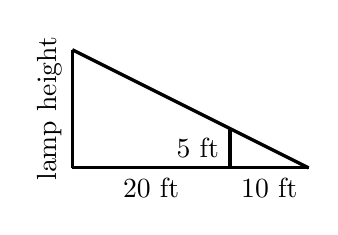
\begin{tikzpicture}

% Define coordinates
\coordinate (O) at (0,0); % Base of the street lamp
\coordinate (P) at (2,0); % Foot of the woman's shadow
\coordinate (Q) at (3,0); % Total shadow
\coordinate (L) at (0,1.5); % Top of the street lamp
\coordinate (M) at (2,0.5); % Top of the woman

% Draw street lamp
\draw[very thick] (O) -- node[midway, above, rotate=90] {lamp height} (L);

% Draw woman
\draw[very thick] (P) -- node[midway, left] {5 ft} (M);

% Label shadow lengths and heights
\draw[very thick] (O) -- node[midway, below] {20 ft} (P);
\draw[very thick] (P) -- node[midway, below] {10 ft} (Q);
\draw[very thick] (L) -- (Q);

\end{tikzpicture}
    \end{center}

    We begin by drawing a rough diagram and labeling the known lengths. In the process of drawing this diagram, we notice there are two triangles, one nested within the other, and they are similar (just like the ones we drew within the circles in the previous exercise). If we can determine the scaling factor between them (or how many times longer the various sides are from one to the other), we can determine the height of the street lamp. \\
    
    Let $x$ represent the height of the street lamp. The base of the larger triangle is 30 feet, and the base of the smaller triangle (which is the length of the woman's shadow) is 10 feet. From these values, we can determine the smaller triangle is scaled by a factor of 3 to achieve the larger triangle. This means that the two heights are also related by a factor of 3. The height of the woman (5 feet) can be scaled up by a factor of 3 to find the height of the street lamp, which means it is 15 feet tall.
    
    We could also determine this using ratios, since similar triangles' respective sides have equal ratios. The ratio of the woman's height to her shadow is equal to the ratio of the height of the street lamp to the base of the larger triangle. From this equation, we can solve for $x$
    \begin{align*}
        \frac{5}{10} &=\frac{x}{30}\\
        30\cdot \frac{5}{10} &= x\\
        15 &= x
    \end{align*}
    Again we find that the height of the street lamp is 15 feet.
\end{solution}
\item 
A water tank is in the shape of a right circular cone with radius 8 feet and height 40 feet. (The tip is at the bottom.) The formula for the volume of a cone with radius $R$ and height $H$ is $V=\frac{1}{3}\pi R^2H$.

  \begin{enumerate}
  \item
    \begin{problem}[\vfill]
      Suppose the tank is filled part-way with water. How are the height of the water and the radius of the surface of the water related?
    \end{problem}

    \begin{solution}

      We start by drawing a picture and labeling important quantities.
      \begin{center} 
        \begin{tikzpicture}[scale =1.3]
          \draw[dashed, ] (0, 0) arc (170:10:2cm and 0.4cm)coordinate[pos=0] (a);
          \draw [] (0, 0) arc (-170:-10:2cm and 0.4cm)coordinate (b);
          \draw[densely dashed, ] ([yshift=-4cm]$(a)!0.5!(b)$) -- node[right, font=\footnotesize] {$40$ feet}coordinate[pos =.95] (aa)($(a)!0.5!(b)$)
          -- node[above , font=\footnotesize] {$10$ feet}coordinate[pos=0.1] (bb) (b);
          \draw [] (aa) -| (bb);
          \draw [](a) -- ([yshift=-4cm]$(a)!0.5!(b)$) -- (b);
        \end{tikzpicture}
        % \begin{tikzpicture}[scale =1.3]
        %   
        %   \draw[dashed, red] (0, 0) arc (170:10:2cm and 0.4cm)coordinate[pos=0] (a);
        %   \draw[dashed, red] (1, -2) arc (170:10:1cm and 0.2cm)coordinate[pos=0] (d) ;
        %   \draw [red] (1, -2) arc (-170:-10:1cm and 0.4cm)coordinate (c);
        %   \draw [red] (0, 0) arc (-170:-10:2cm and 0.4cm)coordinate (b);
        %   \draw[densely dashed, red] ([yshift=-4cm]$(d)!0.5!c)$) -- node[right, font=\footnotesize] {$40$ feet}coordinate[pos =.95] (aa)($(a)!0.5!(b)$)
        %   -- node[above , font=\footnotesize] {$10$ feet}coordinate[pos=0.1] (bb) (b);
        %   \draw [red] (aa) -| (bb);
        %   \draw [red](a) -- ([yshift=-4cm]$(a)!0.5!(b)$) -- (b);
        % \end{tikzpicture}
      \end{center} 

      Let $h$ be the height of the water and $r$ be the radius of the
      surface area of the water.  By similar triangles, $\frac{r}{h} =
      \frac{8}{40} = \frac{1}{5}$.  So, $h = 5r$ or $\frac{h}{5}=r$.
    \end{solution}

    \item
    \begin{problem}[\stretch{2}]
        At this instant, the height of the water in the tank is 10 feet, and water is flowing in at a rate of 16 cubic feet per second. How fast is the height of the water in the tank changing?
    \end{problem}

    \begin{solution}
        Initially, it's helpful to review the prompt and identify the rates and quantities that have been given to us. At the relevant moment in time, the height of water in the tank is 10 feet, so $h=10$, and water is flowing into the tank at a rate of 16 cubic feet per second. Since cubic feet is a unit of volume and seconds are units of time, we identify this as $\diff{V}{t}=16$. When asked how fast the height of the water in the tank is changing, that's asking for $\diff{h}{t}$. 

        We know that volume of a right circular cone is $V=\frac{1}{3}\pi R^2 H$. This equation as it is written is challenging. We have no information about the radius at the moment in question $r$, how big the radius is or how fast it is changing. And so the presence of $r$ adds extra unknowns on top of what we are searching for in this problem ($\diff{h}{t}$), which will make solving impossible. 

        We know the relationship between $h$ and $r$ is $r=\frac{h}{5}$. Substituting this into our volume equation eliminates $r$ and leaves us with only a relationship between $V$ and $h$.
        \begin{align*}
            V&=\frac{1}{3}\pi r^2  h\\
            V&= \frac{1}{3} \pi \bigg(\frac{h}{5}\bigg)^2h\\
            V&= \frac{\pi h^3}{75}\\
            \end{align*}
            Since we are looking for $\diff{h}{t}$, 
            we will differentiate both sides with respect to time to introduce this term, giving us\\
            
            \begin{align*}
            \diff{V}{t}&=\frac{3\pi h^2}{75}\cdot\diff{h}{t}\\
            \diff{V}{t}&=\frac{\pi h^2}{25}\cdot\diff{h}{t}\\
            \end{align*}
            We can now set $h=10$, $\diff{V}{t}=16$, which allows us to solve for our remaining unknown $\diff{h}{t}$\\
            \begin{align*}
            16 &=\frac{\pi (10)^2}{25}\cdot\diff{h}{t}\\
            16&=4\pi\cdot \diff{h}{t}\\
            \frac{4}{\pi}&=\diff{h}{t} 
        \end{align*}
        The height of the water is increasing at a rate of $\frac{4}{\pi}$ feet per second.
    \end{solution}
\end{enumerate}

\end{enumerate}
\end{document}